\documentclass[11pt,a4paper]{report}
\usepackage[textwidth=37em,vmargin=30mm]{geometry}
\usepackage{calc,xunicode,amsmath,amssymb,paralist,enumitem,tabu,booktabs,datetime2,xeCJK,xeCJKfntef,listings}
\usepackage{tocloft,fancyhdr,tcolorbox,xcolor,graphicx,eso-pic,xltxtra,xelatexemoji}

\newcommand{\envyear}[0]{2025}
\newcommand{\envdatestr}[0]{2025-06-17}
\newcommand{\envfinaldir}[0]{webdb/2025/20250617/final}

\usepackage[hidelinks]{hyperref}
\hypersetup{
    colorlinks=false,
    pdfpagemode=FullScreen,
    pdftitle={Web Digest - \envdatestr}
}

\setlength{\cftbeforechapskip}{10pt}
\renewcommand{\cftchapfont}{\rmfamily\bfseries\large\raggedright}
\setlength{\cftbeforesecskip}{2pt}
\renewcommand{\cftsecfont}{\sffamily\small\raggedright}

\setdefaultleftmargin{2em}{2em}{1em}{1em}{1em}{1em}

\usepackage{xeCJK,xeCJKfntef}
\xeCJKsetup{PunctStyle=plain,RubberPunctSkip=false,CJKglue=\strut\hskip 0pt plus 0.1em minus 0.05em,CJKecglue=\strut\hskip 0.22em plus 0.2em}
\XeTeXlinebreaklocale "zh"
\XeTeXlinebreakskip = 0pt


\setmainfont{Brygada 1918}
\setromanfont{Brygada 1918}
\setsansfont{IBM Plex Sans}
\setmonofont{JetBrains Mono NL}
\setCJKmainfont{Noto Serif CJK SC}
\setCJKromanfont{Noto Serif CJK SC}
\setCJKsansfont{Noto Sans CJK SC}
\setCJKmonofont{Noto Sans CJK SC}

\setlength{\parindent}{0pt}
\setlength{\parskip}{8pt}
\linespread{1.15}

\lstset{
	basicstyle=\ttfamily\footnotesize,
	numbersep=5pt,
	backgroundcolor=\color{black!5},
	showspaces=false,
	showstringspaces=false,
	showtabs=false,
	tabsize=2,
	captionpos=b,
	breaklines=true,
	breakatwhitespace=true,
	breakautoindent=true,
	linewidth=\textwidth
}






\newcommand{\coverpic}[2]{
    % argv: itemurl, authorname
    Cover photo by #2~~(\href{#1}{#1})
}
\newcommand{\makeheader}[0]{
    \begin{titlepage}
        % \newgeometry{hmargin=15mm,tmargin=21mm,bmargin=12mm}
        \begin{center}
            
            \rmfamily\scshape
            \fontspec{BaskervilleF}
            \fontspec{Old Standard}
            \fontsize{59pt}{70pt}\selectfont
            WEB\hfill DIGEST
            
            \vfill
            % \vskip 30pt
            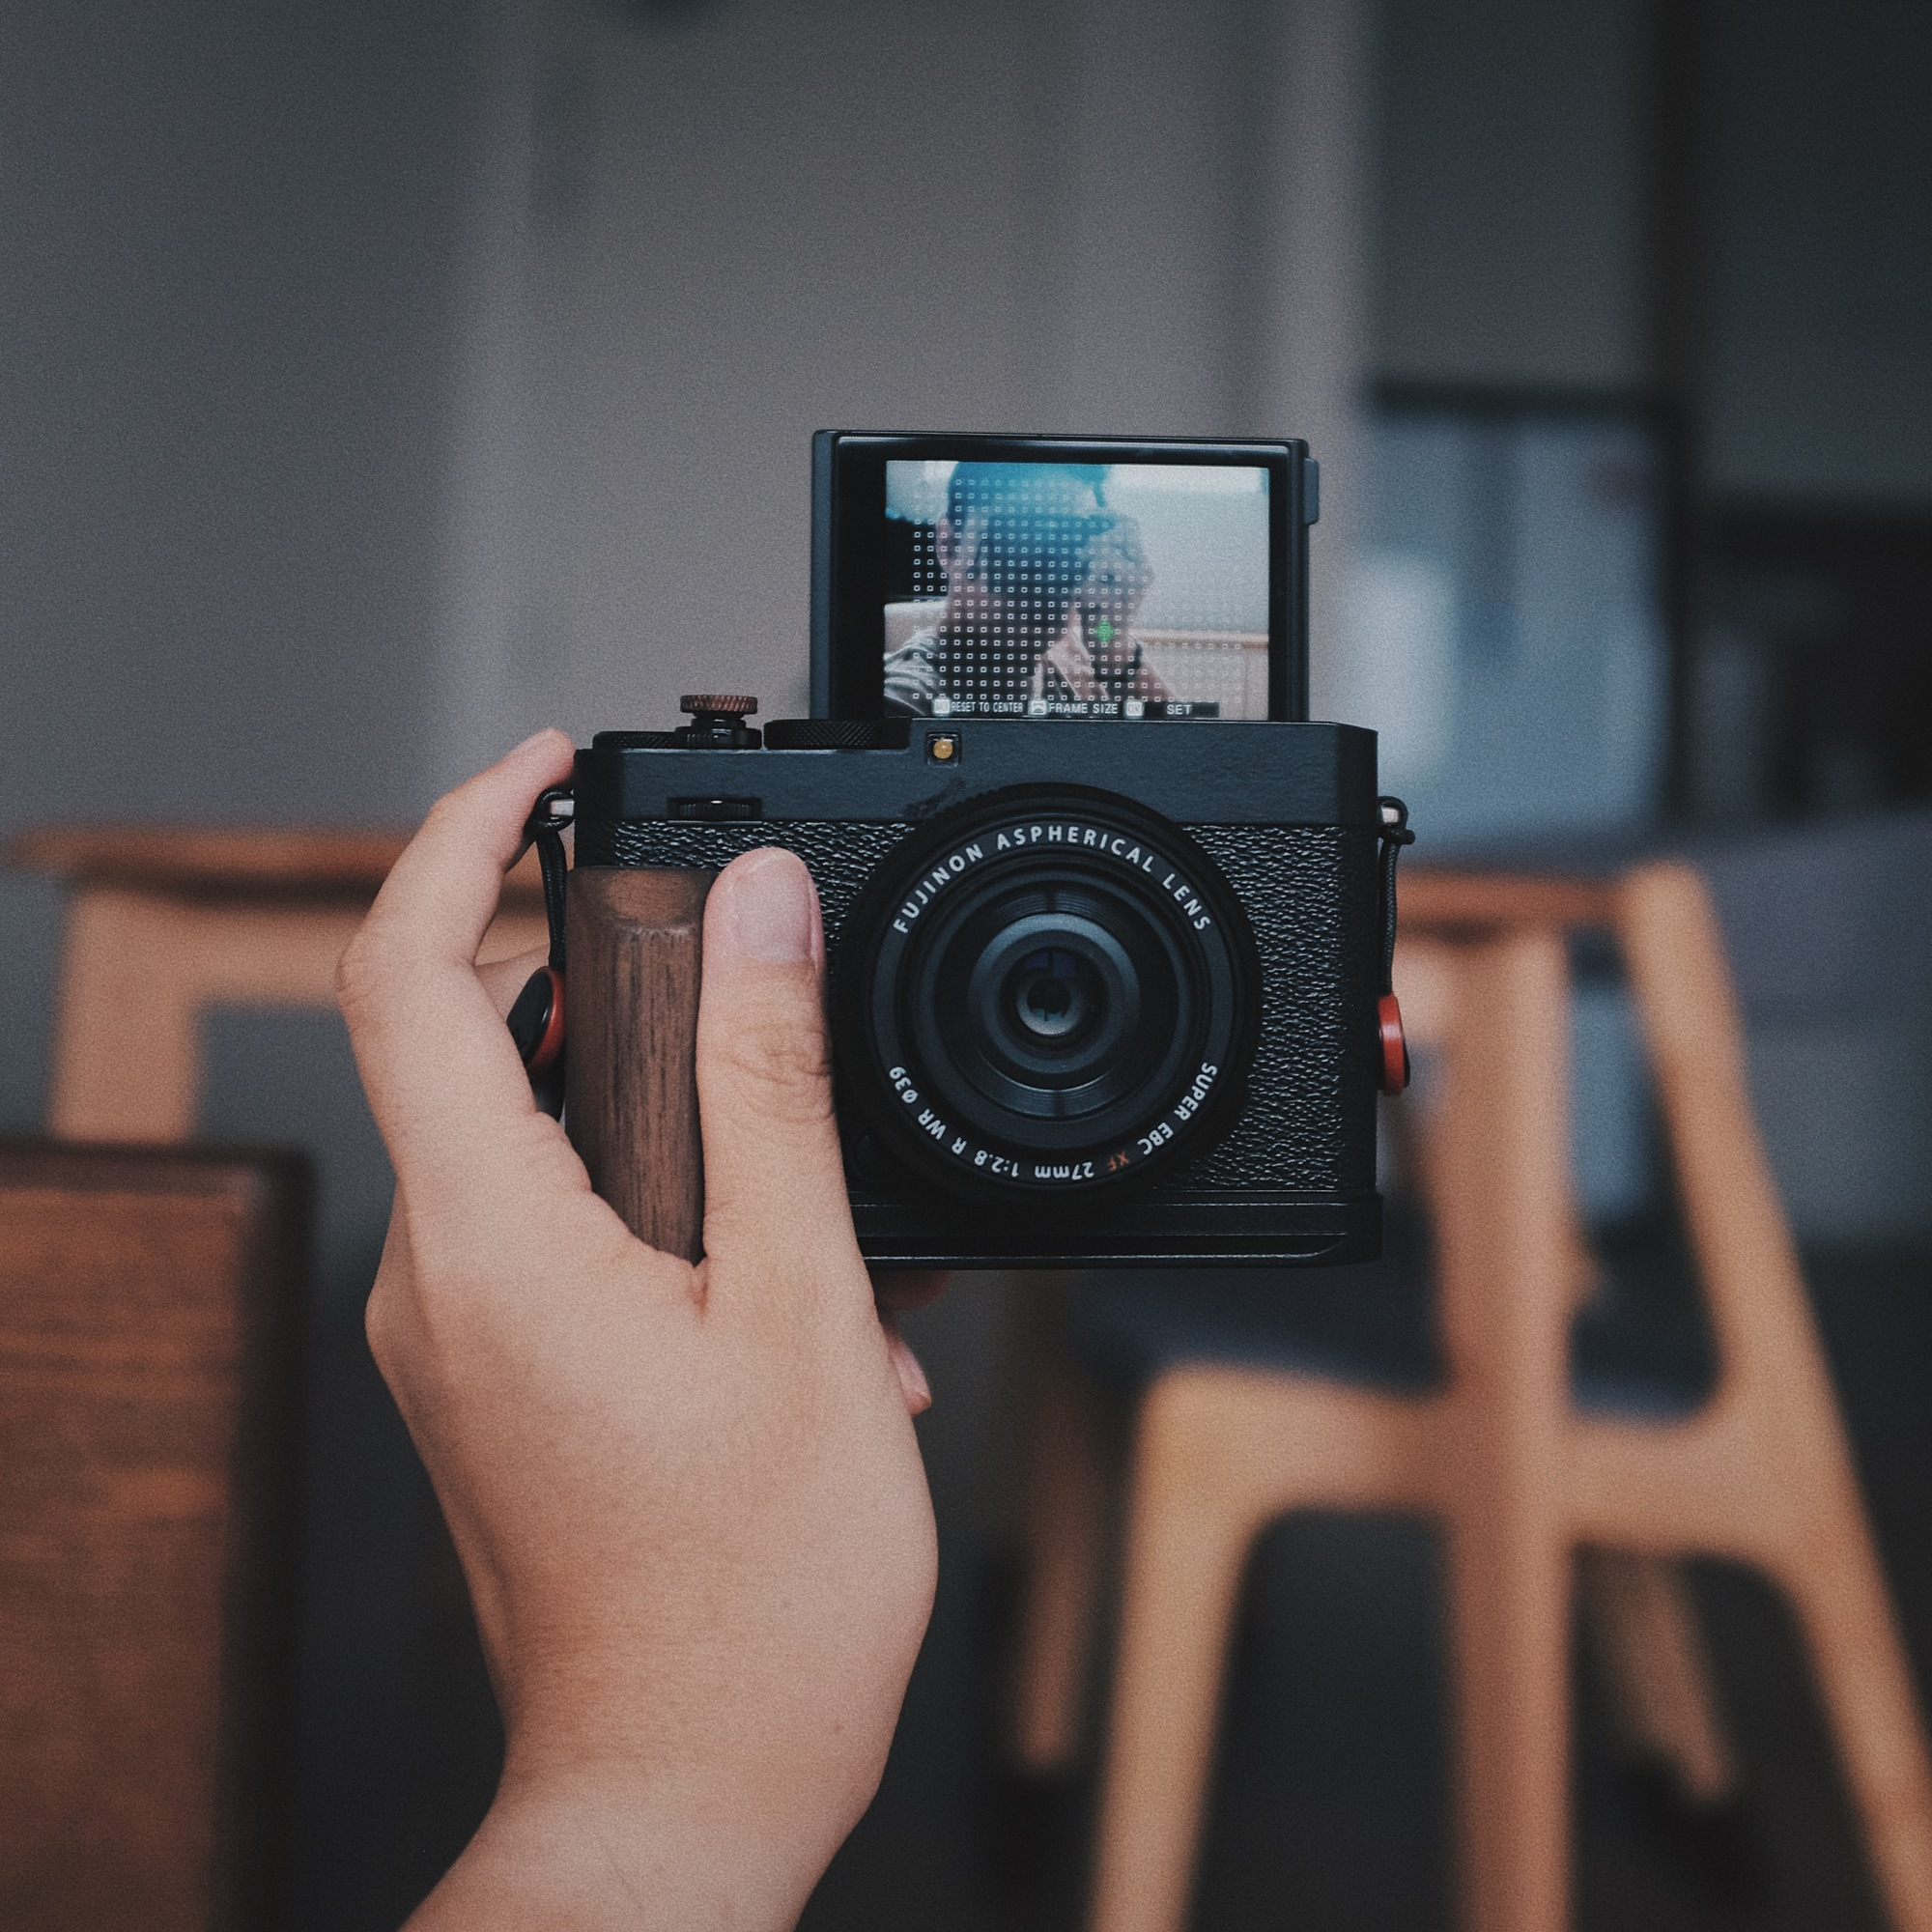
\includegraphics[width=\linewidth]{\envfinaldir/coverpic-prod.jpg}\par
            % \vskip 30pt
            \vfill

            \normalsize\rmfamily\scshape
            \copyright{} The Web Digest Project \hfill\large \envdatestr
        \end{center}
    \end{titlepage}
    % \restoregeometry
}
\newcommand{\simplehref}[1]{%
    \textcolor{blue!80!green}{\href{#1}{#1}}%
}
\renewcommand{\contentsname}{\center\Huge\sffamily\bfseries Contents\par\vskip 20pt}
\newcounter{ipartcounter}
\setcounter{ipartcounter}{0}
\newcommand{\ipart}[1]{
    % \vskip 20pt
    \clearpage
    \stepcounter{ipartcounter}
    \phantomsection
    \addcontentsline{toc}{chapter}{#1}
    % \begin{center}
    %     \Huge
    %     \sffamily\bfseries
    %     #1
    % \end{center}
    % \vskip 20pt plus 7pt
}
\newcounter{ichaptercounter}
\setcounter{ichaptercounter}{0}
\newcommand{\ichapter}[1]{
    % \vskip 20pt
    \clearpage
    \stepcounter{ichaptercounter}
    \phantomsection
    \addcontentsline{toc}{section}{\numberline{\arabic{ichaptercounter}}#1}
    \begin{center}
        \Huge
        \sffamily\bfseries
        #1
    \end{center}
    \vskip 20pt plus 7pt
}
\newcommand{\entrytitlefont}[1]{\subsection*{\raggedright\Large\sffamily\bfseries#1}}
\newcommand{\entryitemGeneric}[2]{
    % argv: title, url
    \parbox{\linewidth}{
        \entrytitlefont{#1}\par\vskip 5pt
        \footnotesize\ttfamily\mdseries
        \simplehref{#2}
    }\vskip 11pt plus 11pt minus 1pt
}
\newcommand{\entryitemGithub}[3]{
    % argv: title, url, desc
    \parbox{\linewidth}{
        \entrytitlefont{#1}\par\vskip 5pt
        \footnotesize\ttfamily\mdseries
        \simplehref{#2}\par\vskip 5pt
        \small\rmfamily\mdseries#3
    }\vskip 11pt plus 11pt minus 1pt
}
\newcommand{\entryitemAp}[3]{
    % argv: title, url, desc
    \parbox{\linewidth}{
        \entrytitlefont{#1}\par\vskip 5pt
        \footnotesize\ttfamily\mdseries
        \simplehref{#2}\par\vskip 5pt
        \small\rmfamily\mdseries#3
    }\vskip 11pt plus 11pt minus 1pt
}
\newcommand{\entryitemHackernews}[3]{
    % argv: title, hnurl, rawurl
    % \parbox{\linewidth}{
    %     \entrytitlefont{#1}\par\vskip 5pt
    %     \footnotesize\ttfamily\mdseries
    %     \simplehref{#3}\par
    %     \textcolor{black!50}{\href{#2}{#2}}
    % }\vskip 11pt plus 11pt minus 1pt
    \begin{minipage}{\linewidth}
            \entrytitlefont{#1}\par\vskip 5pt
            \footnotesize\ttfamily\mdseries
            \simplehref{#3}\par
            \textcolor{black!50}{\href{#2}{#2}}
    \end{minipage}\par\vskip 11pt plus 11pt minus 1pt
}







\begin{document}

\makeheader

\tableofcontents\clearpage




\ipart{Developers}
\ichapter{Hacker News}
\entryitemTwoLinks{Show HN: Chawan TUI web browser}{https://news.ycombinator.com/item?id=44293260}{https://chawan.net/news/chawan-0-2-0.html}

\entryitemTwoLinks{Transparent peer review to be extended to all of Nature's research papers}{https://news.ycombinator.com/item?id=44292342}{https://www.nature.com/articles/d41586-025-01880-9}

\entryitemTwoLinks{Show HN: Canine – A Heroku alternative built on Kubernetes}{https://news.ycombinator.com/item?id=44292103}{https://github.com/czhu12/canine}

\entryitemTwoLinks{Getting free internet on a cruise, saving \$170}{https://news.ycombinator.com/item?id=44291630}{https://angad.me/blog/2025/getting-free-cruise-internet/}

\entryitemTwoLinks{Darklang Goes Open Source}{https://news.ycombinator.com/item?id=44290653}{https://blog.darklang.com/darklang-goes-open-source/}

\entryitemTwoLinks{Benzene at 200}{https://news.ycombinator.com/item?id=44290413}{https://www.chemistryworld.com/opinion/benzene-at-200/4021504.article}

\entryitemTwoLinks{Salesforce study finds LLM agents flunk CRM and confidentiality tests}{https://news.ycombinator.com/item?id=44289554}{https://www.theregister.com/2025/06/16/salesforce\_llm\_agents\_benchmark/}

\entryitemTwoLinks{WhatsApp introduces ads in its app}{https://news.ycombinator.com/item?id=44289412}{https://www.nytimes.com/2025/06/16/technology/whatsapp-ads.html}

\entryitemTwoLinks{Working on databases from prison}{https://news.ycombinator.com/item?id=44288937}{https://turso.tech/blog/working-on-databases-from-prison}

\entryitemTwoLinks{Snorting the AGI with Claude Code}{https://news.ycombinator.com/item?id=44288377}{https://kadekillary.work/blog/\#2025-06-16-snorting-the-agi-with-claude-code}

\entryitemTwoLinks{Tesla blows past stopped school bus and hits kid-sized dummies in FSD tests}{https://news.ycombinator.com/item?id=44288000}{https://www.engadget.com/transportation/tesla-blows-past-stopped-school-bus-and-hits-kid-sized-dummies-in-full-self-driving-tests-183756251.html}

\entryitemTwoLinks{Start your own Internet Resiliency Club}{https://news.ycombinator.com/item?id=44287395}{https://bowshock.nl/irc/}

\entryitemTwoLinks{Nanonets-OCR-s – OCR model that transforms documents into structured markdown}{https://news.ycombinator.com/item?id=44287043}{https://huggingface.co/nanonets/Nanonets-OCR-s}

\entryitemTwoLinks{Accumulation of cognitive debt when using an AI assistant for essay writing task}{https://news.ycombinator.com/item?id=44286277}{https://arxiv.org/abs/2506.08872}

\entryitemTwoLinks{Is gravity just entropy rising? Long-shot idea gets another look}{https://news.ycombinator.com/item?id=44285874}{https://www.quantamagazine.org/is-gravity-just-entropy-rising-long-shot-idea-gets-another-look-20250613/}

\entryitemTwoLinks{Jokes and Humour in the Public Android API}{https://news.ycombinator.com/item?id=44285781}{https://voxelmanip.se/2025/06/14/jokes-and-humour-in-the-public-android-api/}

\entryitemTwoLinks{DARPA program sets distance record for power beaming}{https://news.ycombinator.com/item?id=44285440}{https://www.darpa.mil/news/2025/darpa-program-distance-record-power-beaming}

\entryitemTwoLinks{Real-time CO2 monitoring without batteries or external power}{https://news.ycombinator.com/item?id=44285392}{https://news.kaist.ac.kr/newsen/html/news/?mode=V\&mng\_no=47450}

\entryitemTwoLinks{David Attenborough at 99: 'I will not see how the story ends'}{https://news.ycombinator.com/item?id=44285054}{https://www.thetimes.com/life-style/celebrity/article/david-attenborough-book-extract-age-99-lj3rd2fg7}

\entryitemTwoLinks{Show HN: Zeekstd – Rust Implementation of the ZSTD Seekable Format}{https://news.ycombinator.com/item?id=44284871}{https://github.com/rorosen/zeekstd}\ichapter{Dribbble}
\entryitemGeneric{\hskip 0pt{}Aquasan}{https://dribbble.com/shots/26100535-Aquasan}

\entryitemGeneric{\hskip 0pt{}Eagle}{https://dribbble.com/shots/26099428-Eagle}

\entryitemGeneric{\hskip 0pt{}Mnp Technologies - Logo Design}{https://dribbble.com/shots/26092034-Mnp-Technologies-Logo-Design}

\entryitemGeneric{\hskip 0pt{}Singular Logo Concept (Unused)}{https://dribbble.com/shots/26091755-Singular-Logo-Concept-Unused}

\entryitemGeneric{\hskip 0pt{}Cre8tera // Website}{https://dribbble.com/shots/26091009-Cre8tera-Website}

\entryitemGeneric{\hskip 0pt{}Cool Pool Logo Design - Letter C Monogram}{https://dribbble.com/shots/26091401-Cool-Pool-Logo-Design-Letter-C-Monogram}

\entryitemGeneric{\hskip 0pt{}Gorilla + Bar Chart Logo}{https://dribbble.com/shots/26092670-Gorilla-Bar-Chart-Logo}

\entryitemGeneric{\hskip 0pt{}zeero logo design}{https://dribbble.com/shots/26087342-zeero-logo-design}

\entryitemGeneric{\hskip 0pt{}Create email inbox composition}{https://dribbble.com/shots/26083118-Create-email-inbox-composition}

\entryitemGeneric{\hskip 0pt{}Shori Brand}{https://dribbble.com/shots/26088139-Shori-Brand}

\entryitemGeneric{\hskip 0pt{}Roaring Bear}{https://dribbble.com/shots/26087788-Roaring-Bear}

\entryitemGeneric{\hskip 0pt{}Eagle}{https://dribbble.com/shots/26085536-Eagle}

\entryitemGeneric{\hskip 0pt{}Hand-drawn illustration pack}{https://dribbble.com/shots/26084735-Hand-drawn-illustration-pack}

\entryitemGeneric{\hskip 0pt{}Dog Mascot Various Poses}{https://dribbble.com/shots/26087977-Dog-Mascot-Various-Poses}

\entryitemGeneric{\hskip 0pt{}Branding Concept for Europe}{https://dribbble.com/shots/26087652-Branding-Concept-for-Europe}

\entryitemGeneric{\hskip 0pt{}B2B Dashboard \& Web App UI UX Design for Carbon Solutions}{https://dribbble.com/shots/26076624-B2B-Dashboard-Web-App-UI-UX-Design-for-Carbon-Solutions}

\entryitemGeneric{\hskip 0pt{}Patriot Logo Design (Unused for Sale)}{https://dribbble.com/shots/26081047-Patriot-Logo-Design-Unused-for-Sale}

\entryitemGeneric{\hskip 0pt{}Heliopoint}{https://dribbble.com/shots/26081987-Heliopoint}

\entryitemGeneric{\hskip 0pt{}Apple}{https://dribbble.com/shots/26084067-Apple}

\entryitemGeneric{\hskip 0pt{}Illustration}{https://dribbble.com/shots/26083223-Illustration}

\entryitemGeneric{\hskip 0pt{}Europe Logo Animation}{https://dribbble.com/shots/26082596-Europe-Logo-Animation}

\entryitemGeneric{\hskip 0pt{}Arc Logo}{https://dribbble.com/shots/26083648-Arc-Logo}

\entryitemGeneric{\hskip 0pt{}Heyo Turns 2!}{https://dribbble.com/shots/26078572-Heyo-Turns-2}

\entryitemGeneric{\hskip 0pt{}Fox Brand Mascot}{https://dribbble.com/shots/26077954-Fox-Brand-Mascot}


\ipart{Developers~~~~(zh-Hans)}
\ichapter{Solidot}
\entryitemGeneric{\hskip 0pt{}英国连锁店的面部识别系统错误识别一位女性为小偷}{https://www.solidot.org/story?sid=81569}

\entryitemGeneric{\hskip 0pt{}纽约州开始要求雇主披露裁员是否是 AI 导致的}{https://www.solidot.org/story?sid=81568}

\entryitemGeneric{\hskip 0pt{}YouTube 和 Spotify 出现假专辑和 AI 生成音乐 }{https://www.solidot.org/story?sid=81567}

\entryitemGeneric{\hskip 0pt{}Meta 的大模型 Llama 3.1 能回忆《哈利波特》第一部 42\% 的内容 }{https://www.solidot.org/story?sid=81566}

\entryitemGeneric{\hskip 0pt{}X.Org Server 项目回滚了大量代码}{https://www.solidot.org/story?sid=81565}

\entryitemGeneric{\hskip 0pt{}女孩的数学表现从上学起开始落后}{https://www.solidot.org/story?sid=81564}

\entryitemGeneric{\hskip 0pt{}吃水果和蔬菜与高质量睡眠相关}{https://www.solidot.org/story?sid=81563}

\entryitemGeneric{\hskip 0pt{}饥饿细菌会杀死并吞食其邻居}{https://www.solidot.org/story?sid=81562}

\entryitemGeneric{\hskip 0pt{}澳大利亚鹦鹉学会开饮水器喝水}{https://www.solidot.org/story?sid=81561}

\entryitemGeneric{\hskip 0pt{}山东傅家遗址确认为母系社会}{https://www.solidot.org/story?sid=81560}

\entryitemGeneric{\hskip 0pt{}抓取 Web 内容的 AI 机器人流量难以获利}{https://www.solidot.org/story?sid=81559}

\entryitemGeneric{\hskip 0pt{}人类首次拍摄到太阳南极}{https://www.solidot.org/story?sid=81557}

\entryitemGeneric{\hskip 0pt{}因 AI 科技巨头的间接碳排放自 2020 年以来增长了 50\%}{https://www.solidot.org/story?sid=81556}\ichapter{V2EX}
\entryitemGeneric{\hskip 0pt{}[分享创造] 搞了个 iOS 通过 Wi-Fi 备份到 NAS 的小玩意,分享一下}{https://www.v2ex.com/t/1139025}

\entryitemGeneric{\hskip 0pt{}[问与答] 有台阿里云 ecs9 月到期,什么时候续费划算?}{https://www.v2ex.com/t/1139024}

\entryitemGeneric{\hskip 0pt{}[Chrome] Chrome 的翻译也太烂了吧}{https://www.v2ex.com/t/1139023}

\entryitemGeneric{\hskip 0pt{}[硬件] 5090 怎么最大化利用}{https://www.v2ex.com/t/1139022}

\entryitemGeneric{\hskip 0pt{}[问与答] 求助, PC 显示器与主机远程连接有什么方案?}{https://www.v2ex.com/t/1139020}

\entryitemGeneric{\hskip 0pt{}[Apple] 有人发现 iPad safari 浏览器的场景选择吗?每个场景的 safari 都是独立的 cookies}{https://www.v2ex.com/t/1139019}

\entryitemGeneric{\hskip 0pt{}[分享发现] 失业程序员来柬埔寨创业记录}{https://www.v2ex.com/t/1139018}

\entryitemGeneric{\hskip 0pt{}[分享发现] Github \& Hack Club 青少年编码活动 送免费贴纸 敲代码得奖品}{https://www.v2ex.com/t/1139017}

\entryitemGeneric{\hskip 0pt{}[推广] 我的网站}{https://www.v2ex.com/t/1139016}

\entryitemGeneric{\hskip 0pt{}[深圳] 转租深圳南山区后海名苑居规则 2 房}{https://www.v2ex.com/t/1139015}

\entryitemGeneric{\hskip 0pt{}[分享发现] Next.js 面试题: API 深度解析}{https://www.v2ex.com/t/1139014}

\entryitemGeneric{\hskip 0pt{}[问与答] 什么时候可以做空泡泡玛特}{https://www.v2ex.com/t/1139013}

\entryitemGeneric{\hskip 0pt{}[问与答] 小米手机已经开启 usb 调试,但是要进行 adb 点击,必须得登录小米账号?}{https://www.v2ex.com/t/1139011}

\entryitemGeneric{\hskip 0pt{}[分享发现] 离谱的淘宝售后体验}{https://www.v2ex.com/t/1139010}

\entryitemGeneric{\hskip 0pt{}[分享创造] [独立开发] 做了个极简的一次性投资回报率计算工具,免费!欢迎试用提意见}{https://www.v2ex.com/t/1139009}

\entryitemGeneric{\hskip 0pt{}[云计算] 腾讯云,对于被微信判断为恶意或则色情的网址,有申诉加持吗?}{https://www.v2ex.com/t/1139008}

\entryitemGeneric{\hskip 0pt{}[Discourse] 有个问题,用 Discourse 搭的论坛是不是加载会有点慢}{https://www.v2ex.com/t/1139007}

\entryitemGeneric{\hskip 0pt{}[程序员] 请教一下, 2025 年各位佬选择用什么 Linux 桌面版?从便捷、美观、安全的角度分享一下使用体验.}{https://www.v2ex.com/t/1139005}

\entryitemGeneric{\hskip 0pt{}[职场话题] 远程工作交流群,欢迎加入👏}{https://www.v2ex.com/t/1139004}

\entryitemGeneric{\hskip 0pt{}[程序员] 问下如果要同时管理多台服务器集群,有没有类似 1Panel 这样的}{https://www.v2ex.com/t/1139002}

\entryitemGeneric{\hskip 0pt{}[程序员] 我用 nodejs 开发了个 mcp 工具,现在有个问题}{https://www.v2ex.com/t/1139001}

\entryitemGeneric{\hskip 0pt{}[职场话题] 创业一年后被迫找工作顺利找到}{https://www.v2ex.com/t/1139000}

\entryitemGeneric{\hskip 0pt{}[宽带症候群] [求助]ikuai 和小米 Ax3000 拨号延迟差距问题排查。}{https://www.v2ex.com/t/1138999}

\entryitemGeneric{\hskip 0pt{}[酷工作] [携程 Trip.com] 内推|资深前端|酒店研发|上海|团队技术氛围浓厚}{https://www.v2ex.com/t/1138997}

\entryitemGeneric{\hskip 0pt{}[程序员] PromptX 女娲| 使用 AI 创造 AI}{https://www.v2ex.com/t/1138995}

\entryitemGeneric{\hskip 0pt{}[程序员] 这个 MCP 导航网站推荐优质 MCP?}{https://www.v2ex.com/t/1138994}

\entryitemGeneric{\hskip 0pt{}[职场话题] 想问下上家从来没涨过工资,找工作时下家总是要根据上家给的薪资来决定当前薪资,要怎么解}{https://www.v2ex.com/t/1138993}

\entryitemGeneric{\hskip 0pt{}[信息安全] 中国电信是有什么漏洞被人利用了吗?被几百个连贯的电信 ip 持续攻击}{https://www.v2ex.com/t/1138992}

\entryitemGeneric{\hskip 0pt{}[阅读] DDD 阅读小组纳新}{https://www.v2ex.com/t/1138988}

\entryitemGeneric{\hskip 0pt{}[求职] 求一份实习的工作,软件方面的}{https://www.v2ex.com/t/1138987}

\entryitemGeneric{\hskip 0pt{}[Windows] Win11 不明原因卡顿,重启都不能恢复}{https://www.v2ex.com/t/1138985}

\entryitemGeneric{\hskip 0pt{}[硬件] Nas 硬盘扩容请教}{https://www.v2ex.com/t/1138984}

\entryitemGeneric{\hskip 0pt{}[问与答] 2025 了网站还可能靠 Google Adsense 赚美刀吗…}{https://www.v2ex.com/t/1138983}

\entryitemGeneric{\hskip 0pt{}[酷工作] [杭州全职] [B 端产品经理] 区块链自托管基础设施,负责人直招}{https://www.v2ex.com/t/1138981}

\entryitemGeneric{\hskip 0pt{}[分享创造] 花 1 年时间开发迭代的 ssh 工具,欢迎各位大佬看看怎么样}{https://www.v2ex.com/t/1138980}

\entryitemGeneric{\hskip 0pt{}[问与答] 地图 App 怎么设置混搭出行方式}{https://www.v2ex.com/t/1138979}

\entryitemGeneric{\hskip 0pt{}[程序员] 突然发现自己的 alist 被刷流量了}{https://www.v2ex.com/t/1138978}

\entryitemGeneric{\hskip 0pt{}[投资] 有个事很疑惑,是不潜在被骗}{https://www.v2ex.com/t/1138977}

\entryitemGeneric{\hskip 0pt{}[问与答] 我的关于城乡对立的观点,求破大防。起因是今天在知乎上刷到个有很多城乡对立的回答的问题,不适,然后思考了一下。}{https://www.v2ex.com/t/1138976}

\entryitemGeneric{\hskip 0pt{}[Android] 一加买国际版, 在天猫,京东 可以买得到吗?先不考虑闲鱼了}{https://www.v2ex.com/t/1138975}

\entryitemGeneric{\hskip 0pt{}[上海] 发上海那里看肝癌好?}{https://www.v2ex.com/t/1138973}

\entryitemGeneric{\hskip 0pt{}[职场话题] 北京巨坑公司,大家入职小心!我把公司名发出来各位注意}{https://www.v2ex.com/t/1138972}

\entryitemGeneric{\hskip 0pt{}[分享创造] [个人项目] 我创造了一个``有自己生活''的 AI 伴侣,想邀请你成为她的朋友}{https://www.v2ex.com/t/1138970}

\entryitemGeneric{\hskip 0pt{}[宽带症候群] 为什么手机能打开诈骗网站,电脑却不能}{https://www.v2ex.com/t/1138969}

\entryitemGeneric{\hskip 0pt{}[宽带症候群] 移动宽带被莫名其妙限到 5M 上传了}{https://www.v2ex.com/t/1138968}

\entryitemGeneric{\hskip 0pt{}[生活] 唉,我现在感觉这么活着有啥意思你说}{https://www.v2ex.com/t/1138967}

\entryitemGeneric{\hskip 0pt{}[翻译] 我尝试 2 小时上线一个翻译网站}{https://www.v2ex.com/t/1138966}

\entryitemGeneric{\hskip 0pt{}[宽带症候群] 上传被限,听说是因各省运营商自负盈亏,上传流量跨省要给下载方付费,于是限制上传;并用爬虫加大下载,使用某为 SA 封禁大量上传用户}{https://www.v2ex.com/t/1138965}

\entryitemGeneric{\hskip 0pt{}[分享发现] 刺激的小游戏~~}{https://www.v2ex.com/t/1138964}

\entryitemGeneric{\hskip 0pt{}[科技] 使用 OCR 和 LLM 解决实际问题---录屏题目摘录}{https://www.v2ex.com/t/1138963}


\ipart{Generic News}
\ichapter{联合早报}
\entryitemWithDescription{中国特稿:中国AI产业火爆赛道挤 广州新应用要弯道超车}{https://www.zaobao.com/news/china/story20250615-6713243}{借助人工智能(AI)工具,中国广州市一家汽车美容店的运营团队,半小时内生成100多条个性化视频,店员和顾客扫码转发这些视频后,店铺的新客源在那个星期同比增加50\%。 这家小型汽车美容店的三人团队,每天投入少量时间运营社交媒体账号,利用AI工具帮助产出内容,并进行投放与管理等,获客成本远低于传统模式。 这是广州创业公司 ``筷子科技``的一个销售案例……}

\entryitemWithDescription{国民党县市首长首度缺席海峡论坛 陆方赴台参加旅展被拒}{https://www.zaobao.com/news/china/story20250614-6760804}{(台北综合讯)两岸紧张关系持续影响双方交流,台湾在野党国民党的县市首长17年来首度缺席中国大陆主办的海峡论坛,大陆人士赴台参加两岸旅展的申请,也遭到台湾政府拒绝。 据《自由时报》报道,第十七届海峡论坛星期天(6月15日)起在福建举行。国民党籍县市首长首度缺席论坛,也没有派代表参加,国民党历来至少派出副主席层级参与,今年却仅由大陆事务部主任出席,层级明显下降……}

\entryitemWithDescription{中日就军机太平洋险距接触互相指责}{https://www.zaobao.com/news/china/story20250614-6760181}{(北京/东京综合讯)中国双航母编队首次同时现身西太平洋开展训练,一艘航母上起飞的中国战机与日本巡逻机近距离接触,引发两国互相指责。 日本国防部星期三(6月11日)通报,6月7日至8日,日本海上自卫队``P3C''反潜巡逻机在太平洋公海海域对中国航母``山东舰''进行监视时,舰上搭载的歼-15战斗机起飞抵近日本军机,两机在几乎没有高度差的情况下,一度接近至45米……}

\entryitemWithDescription{波音向中国航空公司交付关税战以来首架飞机}{https://www.zaobao.com/news/china/story20250614-6760378}{(上海/香港综合讯)美国波音公司向中国航空公司交付中美关税战4月开打以来的首架飞机,被视作中美寻求缓解贸易紧张局势的和解迹象。 综合第一财经和彭博社报道,波音星期六(6月14日)向上海吉祥航空公司交付了一架全新787-9飞机。 航班追踪网站``Flightradar24''显示,一架吉祥航空的787-9梦想客机星期五(6月13日)从西雅图起飞,前往上海浦东国际机场……}

\entryitemWithDescription{全球最快高铁试跑:运营时速400公里 最快明年投运}{https://www.zaobao.com/news/china/story20250614-6760458}{(武汉讯)全球最快高铁CR450动车组在中国湖北省试跑,试验时速可达450公里,预计最快明年投入运营,商业运营时速为400公里。 据《湖北日报》报道,CR450动车组星期四(6月12日)在湖北开启约半个月的型式试验,为列车后续调试提供数据验证……}

\entryitemWithDescription{美国移民局将122名非法移民遣返中国}{https://www.zaobao.com/news/china/story20250614-6760186}{(华盛顿讯)美国移民和海关执法局(ICE)本月使用一架所谓的``特殊高风险包机``,将122名非法移民遣返中国。 据美国之音报道,ICE官网在6月9日发表的声明中说,该机构6月3日牵头了美国国土安全部的上述遣返行动。 ICE也说,这次用包机遣返的人员包括96名男性和26名女性,年龄在19到68岁之间,他们都已收到来自全美各地ICE拘留中心的最终递解令……}

\entryitemWithDescription{新加坡峇峇娘惹文化风吹进北京首都博物馆}{https://www.zaobao.com/news/china/story20250614-6758890}{``衣服的设计是,一个洋人妇女穿着衫裤,跟妈姐一起出去逛街。我问她为什么会有这样的设计灵感?她说因为小时候由妈姐照顾,所以在订做卡峇雅(Kebaya)时,她要把美好回忆绣在上面。'' 新加坡娘惹服装设计师黄俊荣(Raymond Wong)星期五(6月13日)在北京首都博物馆举行的``峇峇娘惹文化之夜''上,向逾百名出席者介绍他收藏和设计的卡峇雅服饰,以及服饰背后的故事……}

\entryitemWithDescription{杨丹旭:实习医生罗帅宇之死}{https://www.zaobao.com/news/china/story20250614-6735428}{一桩实习医生坠楼案星期五(6月13日)再次引爆中国网络舆论。 案子仿佛是一部悬疑片的开头。去年5月8日,年仅28岁的中南大学湘雅二医院实习医生罗帅宇蹊跷地在医院附近的居民楼坠亡。警方初步认定为自杀,但家属和网民认为,案子疑点重重。 据多家中国媒体报道,罗帅宇的住所内疑似有发生冲突的痕迹,床单凌乱、眼镜碎裂;在无现金支付普及之际,他的随身包内还有约2万5000元(人民币,下同,4500新元)现金……}

\entryitemWithDescription{新闻人间:``汽车狂人''李书福不再建新厂}{https://www.zaobao.com/news/china/story20250614-6725093}{旗下产业上市版图进一步扩张之际,``汽车狂人''李书福决定,不再扩建汽车工厂。 网约车平台``曹操出行''星期二(6月10日)通过香港交易所的上市聆讯,这代表身为公司大股东的李书福,又要收获一家上市公司。 作为中国民营汽车巨头吉利创始人,李书福目前手握吉利汽车、沃尔沃汽车、钱江摩托、力帆科技和极氪等九家上市公司,业务覆盖整车制造、摩托车、智能科技等多个领域……}

\entryitemWithDescription{冲刺罢免行动 赖清德与曹兴诚沈伯洋会面}{https://www.zaobao.com/news/china/story20250613-6733009}{(台北综合讯)全台罢免行动即将迈入冲刺的第三阶段,民进党中央与罢免团体全力备战,身兼该党主席的台湾总统赖清德星期四(6月12日)与罢免领衔人联电创办人曹兴诚、民进党立委沈伯洋会面。 据《上报》报道,曹兴诚5月底曾与民进党秘书长林右昌会面,两人原本要谈第三阶投票合作策略,但不到半小时便不欢而散,曹兴诚致电总统府秘书长潘孟安,要求民进党换个人来谈……}

\entryitemWithDescription{台湾首宗海底电缆刑事案 中国大陆籍船长被判囚三年}{https://www.zaobao.com/news/china/story20250613-6730365}{(台北综合讯)一艘具有陆资背景的多哥共和国籍权宜船,2月涉嫌在台湾海域拖断海底电缆,该案星期四(6月12日)宣判,中国大陆籍船长被判三年有期徒刑。 这是台湾首宗因破坏海底电缆而被刑事定罪的案件……}

\entryitemWithDescription{北京驻港国安公署与香港国安处首次联合执法 约谈六人并禁止离境}{https://www.zaobao.com/news/china/story20250613-6727120}{(香港综合讯)香港国安法实施将满五周年,中国中央政府驻港国安公署与香港警务处国安处星期四(6月12日)首次在港联合执法,调查一起涉及六人及一个组织的国安案件,约谈六人并禁止他们离境。 香港特区政府官网星期四晚公告,六名人士及一个组织涉嫌于2020年11月至2024年6月期间干犯《香港国安法》第29条``勾结外国或者境外势力危害国家安全''罪……}

\entryitemWithDescription{腾讯据报考虑收购韩国游戏公司Nexon}{https://www.zaobao.com/news/china/story20250613-6725872}{(东京彭博电)中国游戏巨头腾讯据报正评估收购韩国游戏公司Nexon的可能性,以进一步巩固其利润丰厚的游戏版图。 知情人士称,腾讯已与Nexon创办人金正宙家族展开接洽,探讨收购Nexon的可能性。金氏家族目前正与顾问评估包括出售股份在内的多种方案。 受此消息带动,Nexon股价在星期五(6月13日)东京股市开盘时一度上涨10\%……}

\entryitemWithDescription{北大清华反对将校内河湖水当非法牟利商品}{https://www.zaobao.com/news/china/story20250613-6723225}{(北京综合讯)中国著名高校北京大学和清华大学表明,反对将校内的河湖水当作非法牟利商品。 被冠以``北大未名湖湖水''\,``清华校河河水''的瓶装水的商品,近期现身网络交易平台,引发社会关注。 北京大学、清华大学相关部门负责人星期五(6月13日)接受新华社访问时指出,校内河湖水是维系良好生态系统的宝贵资源,不应成为用以非法牟利的商品,坚决反对这样的行为。同时,这种行为也违反校园管理相关规定……}

\entryitemWithDescription{中印同意加快推进恢复直航航班}{https://www.zaobao.com/news/china/story20250613-6725018}{(新德里综合讯)中国和印度同意``加快''恢复两国之间自2020年即中断的直航航班,显示双边关系进一步改善,但未公布具体时间表。 据印度外交部官网发布的消息,中国外交部副部长孙卫东星期四(6月12日)到印度进行为期两天的访问,并与印度外交秘书唐勇胜会面。 印度外交部的声明说,双方同意加快推进恢复中国和印度间的直航航班,以及采取切实措施,简化签证手续,并促进两国媒体和智库的交流……}

\entryitemWithDescription{长安汽车高管:中国车企出海面临三大挑战}{https://www.zaobao.com/news/china/story20250612-6713799}{重庆汽车巨头长安汽车高管关鑫指出,中国汽车出口火热,连续六年保持全球第一大汽车出口国地位,但中国车企出海仍面临三大挑战,包括全球政治局势动荡引发的贸易壁垒和关税压力、海外市场对中国汽车品牌信任不足,以及技术和生态的输出瓶颈。 关鑫是长安汽车东南亚事业部副总经理……}

\entryitemWithDescription{台网红``馆长''直播游上海逾43万人同看 破台湾纪录}{https://www.zaobao.com/news/china/story20250612-6713954}{(台北综合讯)自称曾``绿到爆炸''的台湾知名网红``馆长''(本名陈之汉)首次到访中国大陆,直播游上海吸引逾43万人同步在线观看,打破台湾YouTube直播纪录,但各界褒贬不一……}

\entryitemWithDescription{中国大陆科学家开发对台电战兵棋系统}{https://www.zaobao.com/news/china/story20250612-6713718}{(北京讯)中国大陆科学家针对台湾及周边海域开发出``电战兵棋系统'',以纳秒级精度对复杂地貌进行建模,可在普通笔记本电脑上运行。 四川电子科技大学通信抗干扰实验室的邵世海团队,在今年3月的《电子与信息学报》中发表《面向大尺度战场的信道仿真加速算法》一文。 据《南华早报》引述该文提到的兵棋推演场景,解放军如果在台湾西南方向部署移动电子战平台,启动发射机后将发出强烈脉冲打破电磁静默……}

\entryitemWithDescription{马凯硕:美国退出全球化是二战以来全球体系最严峻挑战}{https://www.zaobao.com/news/china/story20250612-6713752}{新加坡前资深外交官马凯硕认为,美国特朗普政府决定退出全球化,可能是全球体系自第二次世界大战以来面临的最严峻挑战,预计今年世界经济增长将低于2.3%,创2008年金融大海啸以来最慢增速。 马凯硕也强调,中国和亚细安两大经济体的良好关系世上少有,面对世界逐渐封闭,双方必须努力维护区域大门保持敞开。 2025陆海财经论坛星期四(6月12日)在乌节泛太平洋酒店举行,聚焦中国产业出海东南亚的趋势……}

\entryitemWithDescription{国民党启动``爱国者行动''反大罢免}{https://www.zaobao.com/news/china/story20250612-6713630}{台湾中央选举委员会拟于七八月举行大罢免投票,在大罢免第二阶段处于全面溃败的在野国民党,宣示启动``爱国者行动''反制。在野民众党也将助其一臂之力,要对总统赖清德投下不信任票。 执政的民进党去年大选失去最大党地位后,在法案和预算都受制于在野党,便筹划大罢免欲夺回席次……}

\entryitemWithDescription{国安法实施五年逾300人被捕 港府:香港仍面对软对抗等风险}{https://www.zaobao.com/news/china/story20250612-6713584}{《香港国安法》实施近五年来,港府共拘捕逾300人,当中165人被定罪。当局强调,目前香港仍面对外部势力干预、软对抗等风险,未来会继续推动与国家安全相关的教育和宣传。 今年6月30日是《香港国安法》颁布实施五周年……}

\entryitemWithDescription{日本军方指中国航母舰载机异常逼近日巡逻机}{https://www.zaobao.com/news/china/story20250612-6705803}{(东京/北京综合讯)中国两艘航母在太平洋等海域开展训练之际,日本军方通报,从其中一艘航母上起飞的中国战斗机异常逼近日本巡逻机。 日本国防部星期三(6月11日)在官网通报,上星期六(7日),一架从中国航母山东舰上起飞的歼-15战斗机,对日本海上自卫队的P-3C巡逻机进行长达约40分钟的跟踪……}

\entryitemWithDescription{新增印尼 中国过境免签政策适用国家增至55国}{https://www.zaobao.com/news/china/story20250612-6709376}{(北京综合讯)中国国家移民管理局星期四(6月12日)宣布,从即日起,将印度尼西亚纳入240小时过境免签政策。 管理局负责人介绍,此举是加强中国与亚细安国家交流合作的重要举措,有助于提升中印两国合作交往良好势头,推动贸易、投资更加便利高效,促进文明互鉴和民心相通。 这项政策适用国家数量由此增至55个。其中,有40个来自欧洲,包括法国、德国、西班牙、英国、意大利、俄罗斯、乌克兰等……}






\clearpage
\leavevmode\vfill
\footnotesize

Copyright \copyright{} 2023-2025 Neruthes and other contributors.

This document is published with CC BY-NC-ND 4.0 license.

The entries listed in this newsletter may be copyrighted by their respective creators.

This newsletter is generated by the Web Digest project.

The newsletters are also delivered via Telegram channel \CJKunderline{\href{https://t.me/webdigestchannel}{https://t.me/webdigestchannel}}.\\
RSS feed is available at \CJKunderline{\href{https://webdigest.pages.dev/rss.xml}{https://webdigest.pages.dev/rss.xml}}.

This newsletter is available in PDF at
\CJKunderline{\href{https://webdigest.pages.dev/}{https://webdigest.pages.dev/}}.

The source code being used to generate this newsletter is available at\\
\CJKunderline{\href{https://github.com/neruthes/webdigest}{https://github.com/neruthes/webdigest}}.

This newsletter is also available in
\CJKunderline{\href{http://webdigest.pages.dev/readhtml/\envyear/WebDigest-20250617.html}{HTML}} and
\CJKunderline{\href{https://github.com/neruthes/webdigest/blob/master/markdown/\envyear/WebDigest-20250617.md}{Markdown}}.


\coverpic{https://unsplash.com/photos/a-vibrant-japanese-street-scene-at-night-XMAbH81gUbQ}{mos design}


\end{document}
